\chapter{Studying non-Faradic reaction in symmetric cell}

Electrochemical double-layer capacitors are a class of energy storage devices characterized by high power and low energy density. The process of storing energy is based on adsorption of ions, a non-Faradic process, which gives the characteristic fast kinetics at the expense of capacity; they also exhibit high self discharge. The capacity is due to the electrode/electrolyte surface area, therefore materials with high porosity are particularly indicated. In this section, it is reported a work on self standing activated carbon electrodes in three-electrode cell. The presence of the reference electrode allows to separate the time-varying impedance of positive and negative electrodes during the operation of the device.
The electrodes where produced by Dr. Nicolò Pianta in the group of Prof. Riccardo Ruffo at the University of Milano-Bicocca. He brought the electrodes in Bremen during his visiting period where we worked in close collaboration on the establishments of the measurement apparatus and software. The results of this project are published as peer-reviewed journal [???] and the data to a public repository [doi: 10.6084/m9.figshare.21082168].

\subsection{Materials and cell assembling}

The porous carbon electrodes where produced according to this pubblication [M. Tribbia, N. Pianta, G. Brugnetti, R. Lorenzi, R. Ruffo, A new double layer supercapacitor made by free-standing activated carbon membranes and highly concentrated potassium acetate solutions, Electrochim. Acta 364 (2020), 137323]. The device stores energy in form of adsorbtion of potassium and fluorine ions \colorbox{BurntOrange}{why???}.  The electrode where cut as disks of a diameter of 12mm. A solution of 10mM of KF was used as electrolyte, soaked into two glass faber separator to complete the cell stack; the pH of the solution is 10.7. The stack was introduced in a T-shaped cell with a Polyether ether ketone (PEEK) body which posses excellent mechanical properties and is resistant to chemicals (aqueous or organic) and compressed between two stainless-steel cylinders. The third entrance of the body was left for the reference electrode, described in the following. 

\subsection{Reference electrode and position in the stack}

\marginpar{
\captionsetup{type=figure}
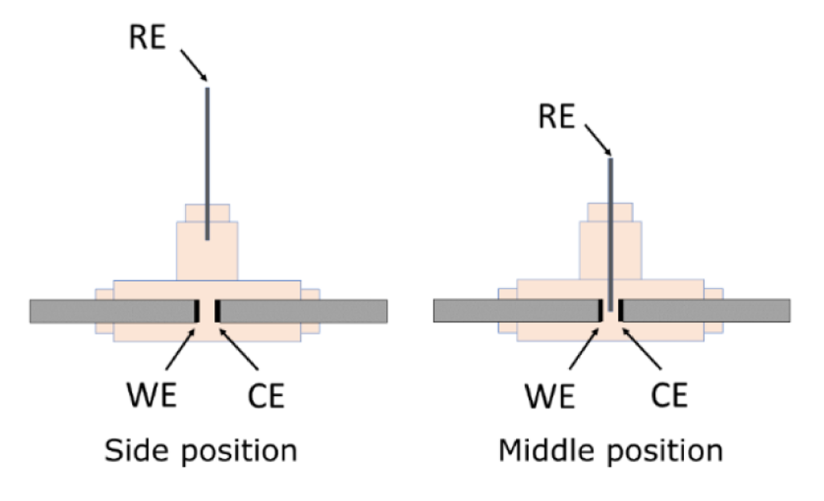
\includegraphics[width=\marginparwidth]{figures/image1.png}
\captionof{figure}{Text of the caption}
}

The geometry of the cell and pH of the electrolytic solution pose a challenge on the choice of the reference electrode. The most common reference electrode for aqueous solutions is AgCl/Ag but its glass encapsulation is too big to be used in a compact systems. A miniaturized electrode must be used for this task which could behave as pseudo-reference electrode in the KF solution. We had to search an element and it halogen that is not soluble in KF solution with a pH of 10.7. The only solution that we found was the red-ox couple PbF2/Pb which produced a stable voltage of 191mV vs RHE. The thermodynamic properties of the materials where deducted from the Porubet diagram at the pH of the solution. It was practical to produce the PbF2 in situ after the introduction of a wire of Pb between the two glass fiber separators. Furthermore we investigate the effect of the position of the reference in the measurement. In fact someone would argue that a commercial AgCl/Ag electrode could be used in this geometry by putting a lot of electrolyte in the body until the level of the liquid would be high enough to accomodate the electrode. We called this a “side position”, where the electrode is posed on the side of the electrodes stack. A schematic is reported in figure ??. A classic EIS measurement immediately shows the insurgent of an artifact due to the position of the reference. The result of the experiment is reported in figure ???.

\marginpar{
    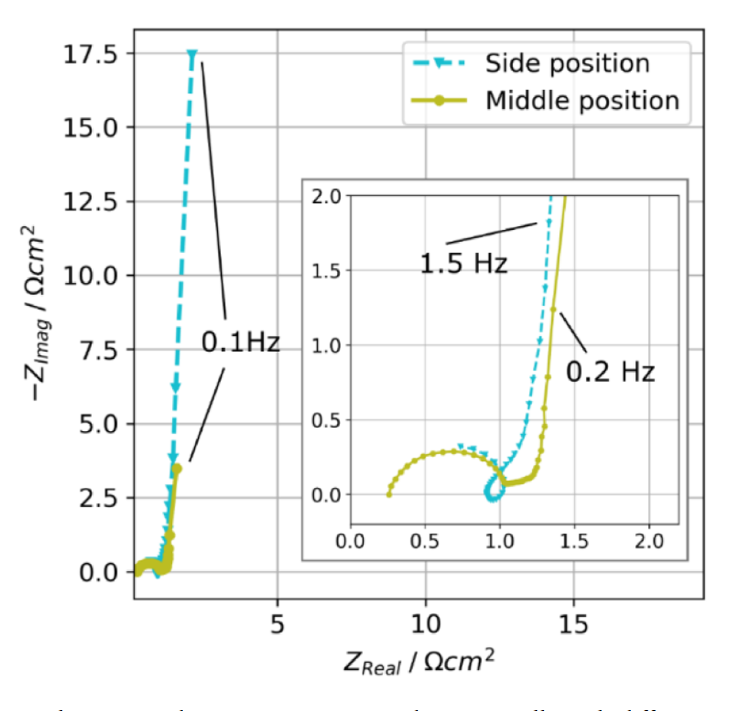
\includegraphics[width=\marginparwidth]{figures/image2.png}
}
I would like to note that also later in the manuscript a wire will be used as reference electrode current collector, but here the entire length of the Pb wire has PbF2 deposited making the electrode surface area quite extensive (while later the wire will be isolated on its length). Nonetheless, the artifacts in the form of a loop in the middle-to-high frequencies are suppress for most of the cases (yes, not completely; cfr. later)  when the reference is in the middle of the cell stack.

\subsection{Physical model}

\subsection{Results and discussions}
We used the Dynamic Multi-Frequency Analysis to estimate the time-varying impedance from 4 consecutive cycles of cyclic voltammetry. !!! parameters used in the DMFA!!! The impedance of the second cycles is reported in figure ???

\begin{figure}[h]
    \centering
    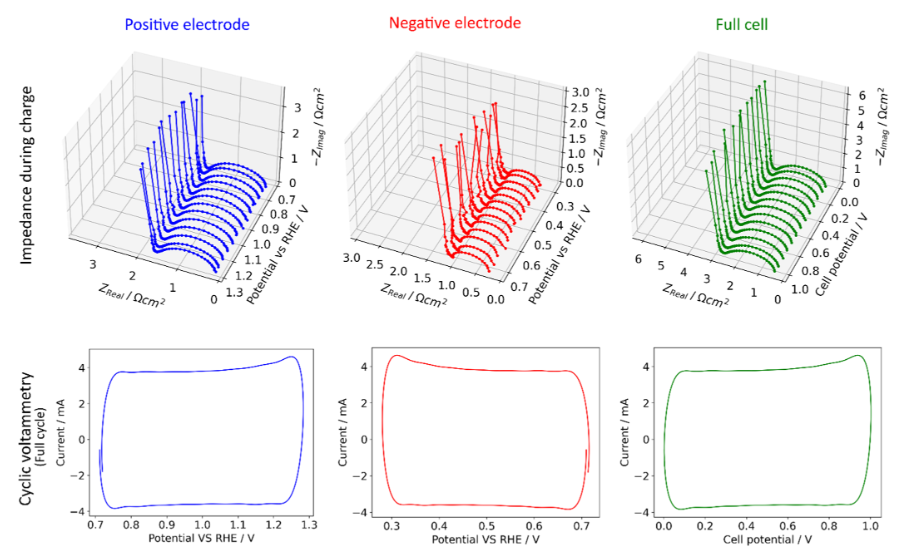
\includegraphics[width = \linewidth]{figures/image3.png}
\end{figure}

The impedance of on helf-cell does not change significantly during the cycle although one can notice some noise in the lowest frequencies for the negative half cell. In the report of the results we omitted the impedance point for the lowest frequency (namely 100 mHz) because it is too much effected by the skirt of the zero frequency and the estimation of the impedance was usefulness; so the figure report the impedance in the interval between 300mHz and 10kHz. In fact, the lowest frequency has to be chosen in relation with the velocity of the dynamic of the system. For examples in this case the system evolves in a bandwidth from 0 to 200mHz. 

Looking at the shape and magnitude of the impedance for the two half-cells in figure ???, it is very interesting to notice the difference of the two interfaces.
\marginpar{
    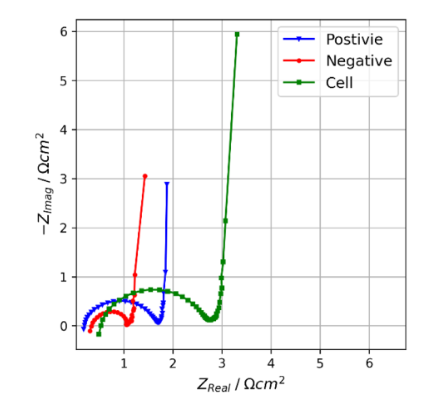
\includegraphics[width=\marginparwidth]{figures/image4.png}
}

Despite the electrodes being chemically identical, the impedance of the two is quite different. We attributed this evidence to the difference in electrode potential, hence the quantity and quality of adsorbed molecules as well as the history of the electrode. The figure show the impedance in the discharge state, where the full cell is almost at 0 V and so the electrical potential of the two interfaces would be the same (around 700mV vs RHE). At the interface, adsorbed molecules can be charged or neutral. In the assumption that both electrodes have the same surface area (being prepared in the same way), we deduce that the nature of adsorbants is different. On the positive electrode in fact, some oxygen anion and oxygen molecule might be still adsorbed at the interface after they are formed in the region between 0.7 and 1 V of the full cell voltage. The presence of elecetrochemical inactive species at the interface would slow down the adsorbtion process of the ions, increasing the interface impedance

From the voltage-time profile of a capacitor one can calculate the average capacitance ????formula???. We found a value of 42 F/g for the positive electrode and 54 F/g for the negative one.

\colorbox{BurntOrange}{Finish the discussion here → take from the paper}

\subsection{Quantitative interpretation of the impedance}

We also analyzed the time-varying impedance through a physical model with the aim of identifying the variation of physical parameter with the time evolution of the system. 

Graphical analysis of the Bode plots?

\subsection{Remarks}

One might argue that the difference in the electrode impedance is not due solely by the history of the electrodes but also the preparation itself. The latter could be identified characterizing more electrodes with the same method. Here the scope of the project was to demonstrate the use of multi-sine non-stationary impedance spectroscopy for characterizing energy storage devices in three-electrode configuration, with less attention on the chemistry. The results where such promising to make us curios of characterizing energy storage devices using non-stationary impedance during galvanostatic drifts, a technique much more appropriate to study such systems. This is the topic of next section.